\chapter[Revisão Bibliográfica]{Revisão Bibliográfica} 
\label{cap:cap2}
%Eu acho que você quis associar o conceito de participação com governança e transparência, acho essa abordagem muito legal. 
%Mas acho que falta você trabalhar um pouco mais essa relação. Pensa que deve existir uma coerência nessa discussão:
%minha sugestão é que você desenvolva melhor o texto seguindo esse caminho: governança digital->transparência->participação

% Introdução do capítulo
Neste capítulo serão discutidos alguns aspectos teóricos necessários para uma boa compreensão do desenvolvimento deste trabalho.

% 1a seção do capítulo 1
\section{Participação Eletrônica e Governança Digital}
\label{sec:e-part}
\par
A utilização de \acrfull{tic} pelo setor público tem transformado a governança global, exigindo de governos e governantes o fornecimento de serviços melhores, 
mais econômicos e eficientes às organizações e indivíduos \cite{afdb2014uneca}. Fatores como o reconhecimento da sociedade civil organizada, o aumento da participação cidadã e a 
ampliação e diversificação dos temas abordados nas esferas governamentais determinaram um novo modelo de governança, a governança digital \cite{o2011government}. 
Este modelo acaba por oferecer um espaço, antes não existente, onde o uso inovador das \acrshort{tic} é a principal ferramenta para ampliar a transparência e participação.

\par
A noção de governança digital é interpretada por \citeonline{reddick2012public} como o resultado da adoção de infraestruturas tecnológicas para a otimização da entrega de 
serviços à população. Ou seja, a utilização de \acrshort{tic} pelo setor público passa a se referir ao modo como as tecnologias e a internet podem melhorar a capacidade do Estado 
de formular e implementar suas políticas públicas \cite{parra2017governancca}. \citeonline{germani2016desafios} complementa a definição de governança digital afirmando que sua 
utilização pelo setor público deve ter o objetivo de melhorar a disponibilização de informações e o fornecimento de serviços públicos aos cidadãos, 
além de incentivar o engajamento da sociedade nos processos políticos, aprimorando os níveis de responsabilidade, transparência e efetividade do governo.

\par
De acordo com o conceito de governança digital apresentado pela \acrshort{onu}, o uso de \acrshort{tic} deve ser definido para atender aos três pilares fundamentais: 
a prestação de melhores serviços pelos agentes públicos, o maior acesso à informação e a maior participação da sociedade civil em todos os ciclos de políticas públicas. 
Dessa forma, \acrshort{tic} representam um papel de catalizadoras desses três pilares podendo obter níveis de desempenho mais satisfatórios \cite{onu2018}. 

\par
Para \cite{rushkoff2003open}, o conceito de governança digital democratiza a tomada de decisão e incentiva a colaboração voluntária entre os indivíduos. 
Diversos paradigmas sobre este modelo de tomada de decisão vêm sendo reexaminados. Além disso, o papel do gestor público e do cidadão têm sido reavaliados pois a incorporação 
de novas tecnologias na relação entre estado e sociedade amplia e possibilita uma outra dinâmica a essa relação. 

\par
Segundo \citeonline{vaz2017transformaccoes}, o crescimento do conceito e da comunidade \textit{open source}, atrelados ao compartilhamento de dados governamentais, 
permite a produção descentralizada de aplicações, serviços e sistemas tecnológicos. Criando assim, o que o autor chama de Segunda Geração de Governança Digital, 
que consiste na busca por iniciativas além das unidirecionais, nas quais o governo apenas disponibiliza os dados captados sobre a população.

\par
Para \citeonline{braga2016participaccao} a possibilidade de um maior acesso às informações e ao conhecimento, permite uma maior transparência nas decisões tomadas por governantes. 
\citeonline{vaz2017transformaccoes} argumenta que há a necessidade de alteração do atual modelo \textit{broadcasting}, para um modelo mais participativo de tomada de decisões. 
Define-se "modelo \textit{broadcasting}", segundo o autor supracitado, como um modelo de alocação dos recursos digitais como recursos secundários ou complementares 
às iniciativas presenciais de relacionamento entre governos e sociedade. Nesse modo, são os governantes que estabelecem os momentos, formatos e conteúdo dos processos 
participativos e de controle social. Isso acaba por restringir as iniciativas apenas às iniciativas governamentais, nas quais a interação e participação nas decisões e no
controle social das políticas públicas são monopolizadas pelo Estado \cite{parra2017governancca}.

\par
Para que haja a evolução desse modelo atual, \citeonline{o2011government} sugere que o governo deve disponibilizar suas informações em uma infraestrutura que permita a sua reutilização
sistemática pela sociedade civil. Ao disponibilizar suas informação, o governo estimula o desenvolvimento de inciativas e ferramentas tecnológicas, ampliando assim a possibilidade 
do uso diverso das informações \cite{zuiderwijk2012socio}. As funções de fazer política e entregar serviços públicos precisam ser reinterpretadas e a participação dos cidadãos
tem que se dar de uma maneira mais ativa \cite{bovaird2007beyond}.

\par
De acordo com a \citeonline{onu2018}, promover essa participação cidadã é fundamental para a governança de uma sociedade civil organizada e inclusiva. O objetivo dessa governança deve
ser direcionado à melhoraria do acesso às informações e aos serviços públicos, pelo incentivo à inclusão do cidadão na tomada de decisões públicas que impactem o bem estar da 
sociedade e do indivíduo em particular.  Neste contexto, surge o conceito de Participação Eletrônica definido por \citeonline{macintosh2008democracy} como o uso de \acrshort{tic}
a fim de ampliar e aprofundar a participação política para que cidadãos sejam capazes de se conectar uns aos outros e aos seus representantes eleitos. 

De acordo com \cite{medeiros2009novos}, o uso das ferramentas de participação eletrônica tem se disseminado para diversos casos de uso e em muitos ambientes diferentes, podendo 
ser encontrados exemplos por todo o mundo. \citeonline{dal2015ferramentas}, por exemplo, mostra em sua pesquisa exploratória sobre inciativas destinadas à participação civil
pela internet, casos de uso de ferramentas de participação eletrônica em Barcelona, Lisboa, São Paulo, Nova Iorque e Porto Alegre. A autora chega a conclusão de 
que o uso de ferramentas de participação eletrônica por governos é um "caminho sem volta".

\par
Contudo, a sociedade civil ainda não tem se engajado plenamente ao uso desses recursos. Para exemplificar, temas de grande interesse popular 
como as reformas trabalhista, tributária e da previdência social brasileira recebem grande atenção dos veículos de comunicação sendo relatados por especialistas como fundamentais 
para o desenvolvimento do país. Portanto, é razoável esperar que que os cidadãos se sintam motivados à participar de discussões voltadas a esses temas. 

\par
Contudo, a ferramenta de participação eletrônica Wikilegis, desenvolvida pela câmara dos deputados do Brasil, disponibilizada em um ambiente virtual onde a sociedade civil pode analisar
 os projetos de leis e contribuir com sugestões para redação aos artigos ou parágrafos, apresenta uma quantidade inexpressiva de sugestões para os projetos de reformas. 
 São 221 sugestões para a reforma da previdência, 129 sugestões para a reforma tributária e  50 sugestões para a reforma trabalhista.  Os números mostram a dificuldade de engajar 
 a sociedade civil em assuntos políticos mais complexos e que demandam tempo e estudo. \textit{Wikilegis}. Disponível em <https://edemocracia.camara.leg.br>. Acesso em 10 out 2018. 

\par
Por outro lado, durante a pesquisa, foi possível encontrar casos onde o engajamento dos cidadãos foi maior. Por exemplo, o site Vote na web disponibiliza um painel, onde são mostrados projetos de leis, 
seus propositores e componentes gráficos para representar a votação dos cidadãos.
Assim, o cidadão pode comparar sua intenção de voto com as dos demais cidadãos e com os votos efetivados pelos representantes, além de contar com a descrição dos votos por gênero,
região e idade. Os projetos têm em média sete mil votos, onde o mais votado conta com cerca de quase quinze mil votos. \textit{Vote na Web}. Disponível em <http://www.votenaweb.com.br/>.
Acesso em 10 out 2018.

\par
Isso indica que o engajamento da sociedade civil organizada tem um amplo espaço de crescimento \cite{o2011government}, fica o desafio aos atores, sociedade civil, governantes, 
empresas e indivíduos, à criação de ferramentas de participação eletrônica que estimulem o engajamento do cidadão.


%=====================================================================================================================================================================================================
% FERRAMENTAS DE PARTICIPAÇÃO ELETRÔNICA
%=====================================================================================================================================================================================================
\newpage
\section{Ferramentas de Participação Eletrônica}
\label{sec:e-part tools}
Devido aos incentivos gerados por esses novos paradigmas de tomada de decisões participativas, muitas ferramentas de participação eletrônica têm sido desenvolvidas,
tanto por governos e governantes, quanto pela sociedade civil organizada. Alguns exemplos de ferramentas de participação eletrônica, levantados
durante esta pesquisa, podem ser encontrados na Tabela \ref{tab:ferramentas}.

\vspace{1cm}

\begin{table}[!ht]
    \centering
    \caption{Ferramentas de Participação Eletrônica}
    \label{tab:ferramentas}
    \begin{tabular}{l*{2}{>{\raggedright\arraybackslash}p{0.5\linewidth}}}
    \toprule
        Nome                             & Acesso                           \\ 
    \midrule
        Crowd For Roads                  & c4rs.eu                          \\
        Decidim Barcelona                & decidim.barcelona                \\
        e-Cidadania                      & senado.leg.br/ecidadania         \\
        Iniciativa de Cidadania Europeia & ec.europa.eu/citizens-initiative \\
        LabRIO                           & lab.rio                          \\
        Mandato Participativo            & saopaulo.sp.leg.br               \\
        Participa.BR                     & participa.br                     \\
        Patio                            & patiolla.fi                      \\
        Plataforma Brasil                & plataformabrasil.org.br          \\
        Portal e-Democracia              & edemocracia.camara.gov.br        \\
        SigaLei                          & sigalei.com.br                   \\
        Visor Urbano                     & visorurbano.com                  \\
        Vote na Web                      & votenaweb.com.br                 \\ 
        We The People                    & petitions.whitehouse.gov         \\
        WeLive                           & welive.eu                        \\
        Wikilegis                        & edemocracia.camara.leg.br        \\
    \bottomrule
    \end{tabular}
\end{table}

As novas tecnologias mostraram uma gama de possibilidades para que os cidadãos ampliem o peso de sua participação nas decisões políticas,
melhorando a capacidade de mobilização, articulação, e possibilitando um maior envolvimento dos atores sociais \cite{araujo2015democracia}.\\

\par
\citeonline{saebo2008shape} dividem os atores sociais em quatro grupos: 

\begin{minipage}{.66\textwidth}	
   \textit{I}) Cidadãos, \\
   \textit{II}) Governantes, \\
   \textit{III}) Instituições estatais e \\
   \textit{IV}) Instituições Voluntárias. \\
\end{minipage}

\par
Esse agrupamento feito pelo autor supracitado é uma abstração da análise de \citeonline{macintosh2006evaluating}, deixando de lado um quinto grupo:

\par
\textit{V}) Provedores de Tecnologia.

\par
Contudo, \citeonline{wimmer2007ontology} agrupa esses atores mais objetivamente, dividindo-os em apenas dois grupos, são eles:\\

\begin{minipage}{.75\textwidth}	
   \textit{a}) Beneficitários da utilização das ferramentas e \\
   \textit{b}) Responsáveis pela administração da ferramenta de participação.  \\
\end{minipage}

\par
Demonstrando uma necessidade e interesse em ferramentas de participação eletrônica, a \acrfull{ocde}, juntamente com a \acrshort{onu} e a \acrfull{ue} criaram o \acrfull{epi}, 
índice que avalia governos frente ao uso de serviços digitais para prover informação aos seus cidadãos, interagir com os atores da sociedade e engajar os cidadãos no processo 
de tomada de decisão. 

\par 
O \acrshort{epi} de um país é composto pelos mecanismos de participação eletrônica que são utilizados pelo governo, comparado relativamente a todos os outros países.
A intenção desse índice não é indicar práticas a serem seguidas, mas sim oferecer um parâmetro geral para que diferentes países possam saber o quanto os governos têm 
feito uso e promovido iniciativas de participação eletrônica \cite{onu2018} .

\par
Diante deste cenário, onde o uso de ferramentas de participação eletrônica está sendo incentivado por instituições, governos e cidadãos, a criação de uma taxonomia para 
classificação de ferramentas de participação eletrônica de maneira colaborativa representa uma possibilidade de elaboração de um instrumento que facilite a compreensão e, 
por consequência, a utilização efetiva dessas ferramentas.

%Livro original do Lineu em LATIN => https://ia800503.us.archive.org/8/items/mobot31753000798865/mobot31753000798865.pdf
%Em Inglês => http://lib1.org/_ads/2AF4FEC3E909EC17EFE5EA7FDA9071E5
%==================================================================================================================================================================================================
\newpage
\section{Taxonomia}
\label{sec:taxonomia}
Com o objetivo de apresentar um panorama conceitual sobre o termo taxonomia e contextualizar o assunto, \citeonline{novo2007elaboraccao} diz que o conceito de taxonomia
não é algo moderno e não emerge instantaneamente como um modelo de solução de problemas de representação do conhecimento sobre um dado domínio. Mas é sim,
o resultado de um extenso processo histórico de estudos e investigações que convergiram para uma construção teórica sobre o assunto. 

\par
O termo taxonomia se origina do grego \textit{taxis} (ordem) e \textit{nomos} (lei, norma) e foi utilizado pela primeira vez em 1735 pelo cientista e médico sueco Carl von Linné,
com a publicação da obra \textit{Systema Naturae}, que contava com apenas 10 páginas em sua primeira edição. Em 1770, em sua 13ª edição, a obra já contava com mais de 3000 páginas.
Durante o século XVIII, Linné classificou os seres vivos de acordo com suas características distintas e os categorizou hierarquicamente, dividindo-os em reinos, filos, classes, ordens, famílias, 
gêneros e espécies, que após algum tempo foram subdivididos. Sua classificação ficou conhecida como “Taxonomia de Lineu” \cite{polaszek2010systema}.

\par
Outro exemplo clássico de taxonomia é a Taxonomia de Bloom, que visa classificar o domínio cognitivo sobre um determinado assunto, e é estudada, principalmente, pelo campo educacional.
\citeonline{ferraz2010taxonomia} mostram que atualmente, o que os pesquisadores chamam de Taxonomia de bloom revisada, é dividida em níveis de complexidade gradualmente crescentes,
onde alguém passando pelo processo de aprendizagem deve progredir na seguinte ordem: Lembrar, entender, aplicar, analisar, sintetizar e por último, criar. Os autores concluíram que 
a taxonomia de bloom colabora para o planejamento, estrutura e organização de cursos, módulos e/ou disciplinas, tanto para estudantes quanto para professores. 


\par
Tradicionalmente utilizada para a classificação das espécies em botânica e zoologia, taxonomias têm sido também utilizadas para estudos da área de Ciência da Informação.
\citeonline{terra2005taxonomia} definem o uso de taxonomias nesse contexto como um instrumento ou elemento de estrutura que permite alocar,
recuperar e comunicar informações dentro de um sistema de maneira lógica.

\par
A utilização de taxonomia nos sistemas de informação não leva em consideração família, gênero ou espécie, como na biologia, mas sim conceitos.
As classes e subclasses de uma taxonomia se apresentam de maneira lógica, suportada por princípios classificatórios.\cite{campos2012taxonomia}
\citeonline{aganette2010elementos} diz que diferente do princípio dicotômico adotado na taxonomia dos seres vivos, atualmente, faz-se possível a construção de taxonomias
policotômicas, ou seja, onde um objeto é classificado em tantas classes, e subclasses quantas necessárias, dentro um domínio especializado.

\par
Sendo assim, é possível utilizar a representação taxonômica da Figura \ref{fig:exemploTaxonomia} para classificar um objeto, arbitrariamente escolhido,
de acordo com os nós F e C, por exemplo.

\begin{figure}[!ht]
\begin{tikzpicture}[level 1/.style={sibling distance=5cm},level 2/.style={sibling distance=2.5cm}]
    \node {T}
        child { node {A}
        child {node{D}}
        child {node{E}}
        child {node{F}}
        child {node{G}}
        child {node{H}}
        }
        child { node {B}}   
        child { node {C}}  
    ;
\end{tikzpicture}
\caption{Exemplo de Taxonomia}
\label{fig:exemploTaxonomia}  
\end{figure}

%==================================================================================================================================================================================================
\subsection{Taxonomia para Ferramentas de Participação Eletrônica}
\label{subsec:taxonomia e-part tools}
\par
Durante esta pesquisa, a revisão da literatura permitiu identificar alguns estudos e ações no sentido de tentar elaborar tipos de classificações para as ferramentas de participação.
Como por exemplo, o projeto \textit{Civic Tech Field Guide}, que atualmente ainda se encontra em estado embrionário, sendo o principal meio de colaboração o preenchimento de um formulário online.
Na seção \ref{subsec:taxonomiaElaborada}, será explicitado o modelo taxonômico adotado por este trabalho.

\par
Taxonomia, no contexto da computação, tem aplicação em distintas áreas. A utilização de estruturas taxonômicas para classificar sistemas, arquiteturas e arquivos data de mais de
cinquenta anos. Uma das classificações taxonômica com maior relevância para a área da computação é a chamada "Taxonomia de Flynn",
onde \citeonline{flynn1966very} classificou as arquiteturas de computadores da seguinte forma:\\

\begin{minipage}{.66\textwidth}
    \begin{singlespace}
        \begin{itemize}
            \item \acrfull{sisd}
            \item \acrfull{simd}
            \item \acrfull{misd}
            \item \acrfull{mimd}
        \end{itemize}
    \end{singlespace}
\end{minipage}
\vspace{0.5cm}

\begin{figure}[!ht]
    \begin{tikzpicture}[level 1/.style={sibling distance=5cm},level 2/.style={sibling distance=2.5cm}]
        \node {T}
            child { node {\acrshort{sisd}}}   
            child { node {\acrshort{simd}}}  
            child { node {\acrshort{misd}}}   
            child { node {\acrshort{mimd}}}  
        ;
    \end{tikzpicture}
    \caption{Taxonomia de Flynn}
    \label{fig:taxonomiaFlynn}  
\end{figure}

\vspace{0.5cm}
\par
Na área de tolerância a falhas, da engenharia de \textit{software}, também é possível encontrar taxonomias. Entre as mais conhecidas estão a taxonomia proposta por
\citeonline{gartner1999fundamentals}, que aborda diversos conceitos e os aplica a um cenário distribuído,
e a taxonomia apresentada por \citeonline{avizienis2004basic}, que define conceitos sobre tolerância a falhas e segurança computacional.

\par
\citeonline{sondhi2018taxonomy} criou uma taxonomia que pode ser usada para prever as ações ou intenções de um usuário em particular de uma dada loja virtual
e então personalizar o algoritmo de busca para indicar as necessidades específicas desse usuário. Vale ressaltar a grande utilização de taxonomia por lojas virtuais, 
e o grande número de trabalhos encontrados, pelo autor, sobre taxonomia aplicada a esse setor de \textit{e-commerce}.

%==================================================================================================================================================================================================
\subsection{Taxonomia Elaborada}
\label{subsec:taxonomiaElaborada}
\par
A taxonomia utilizada como base para construção da ferramenta foi no contexto do projeto Vispublica. Esse trabalho começou com a criação do SOPA que pode ser definido como uma 
ferramenta de participação eletrônica . Esse estudo evoluiu com a elaboração da taxonomia . 

\par
A Taxonomia está representada na Figura \ref{fig:taxonomia-vispublica}, sendo composta por 4 grupos: sustentação, domínio, tecnologias e funcionalidades.
Os grupos são diferenciados por cores e, para cada grupo, foram identificadas classes e subclasses.

\begin{figure}[!ht]
    \centering
    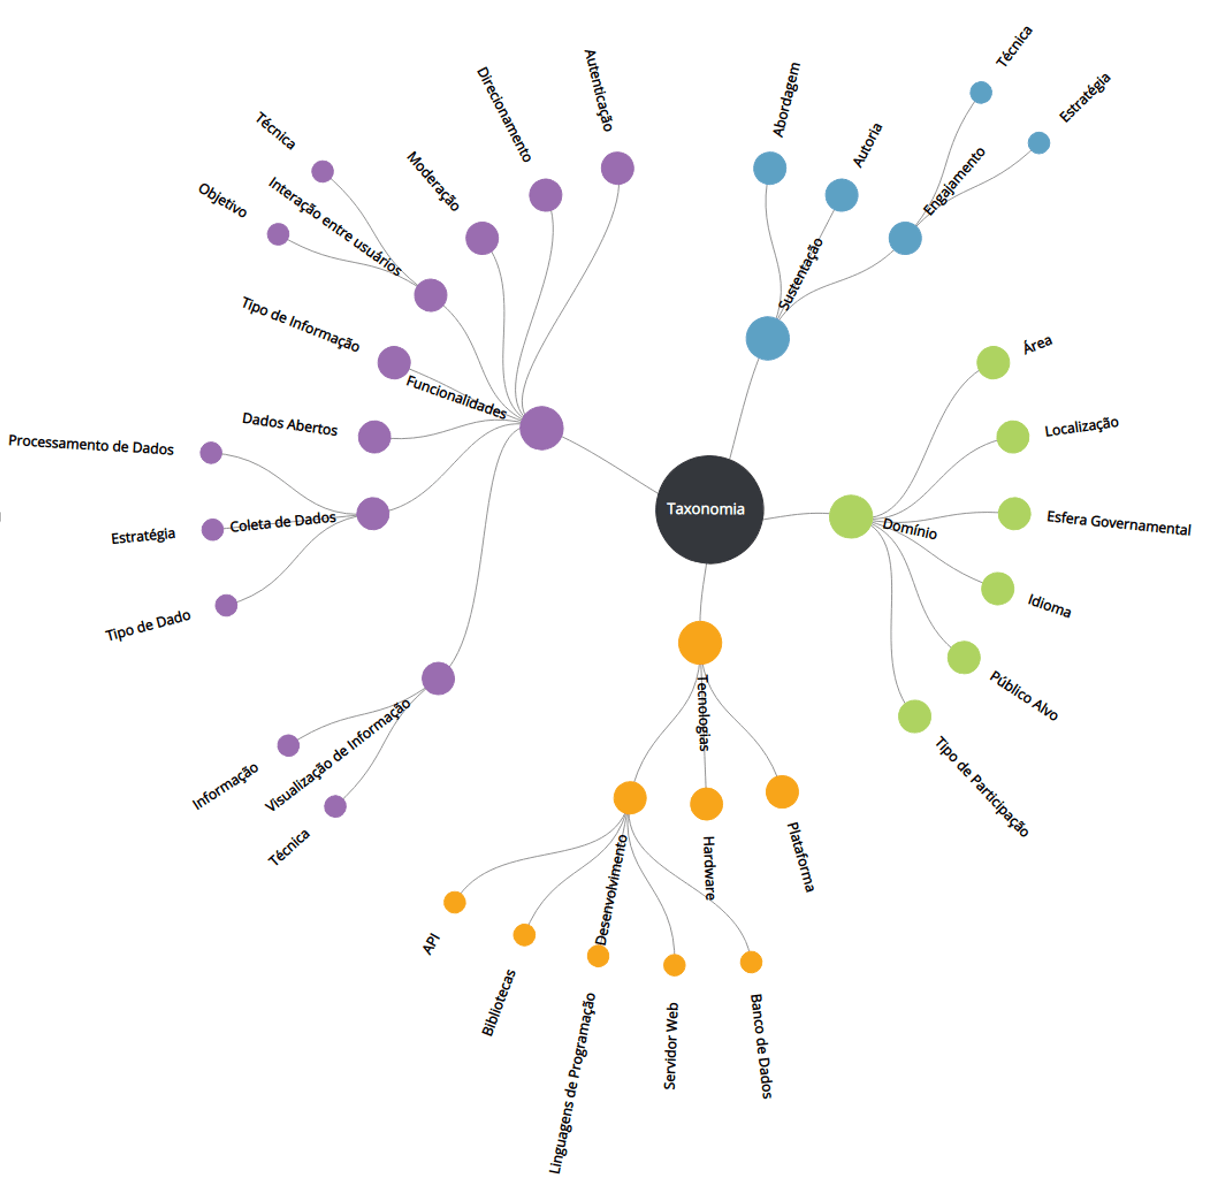
\includegraphics[scale=0.30]{./figuras/taxonopart-radial.png}
    \caption{Taxonomia elaborada pelo projeto Vispública}
    \label{fig:taxonomia-vispublica}
\end{figure}

O grupo sustentação explora as questões relacionadas a como e quem promove a ferramenta de forma que seja utilizada, ou seja, como se dá a sustentabilidade da ferramenta. 
Na Figura \ref{fig:grupo-sustentacao} é possível observar a hierarquia para classificação definida no grupo sustentação.

\begin{figure}[!ht]
    \centering
    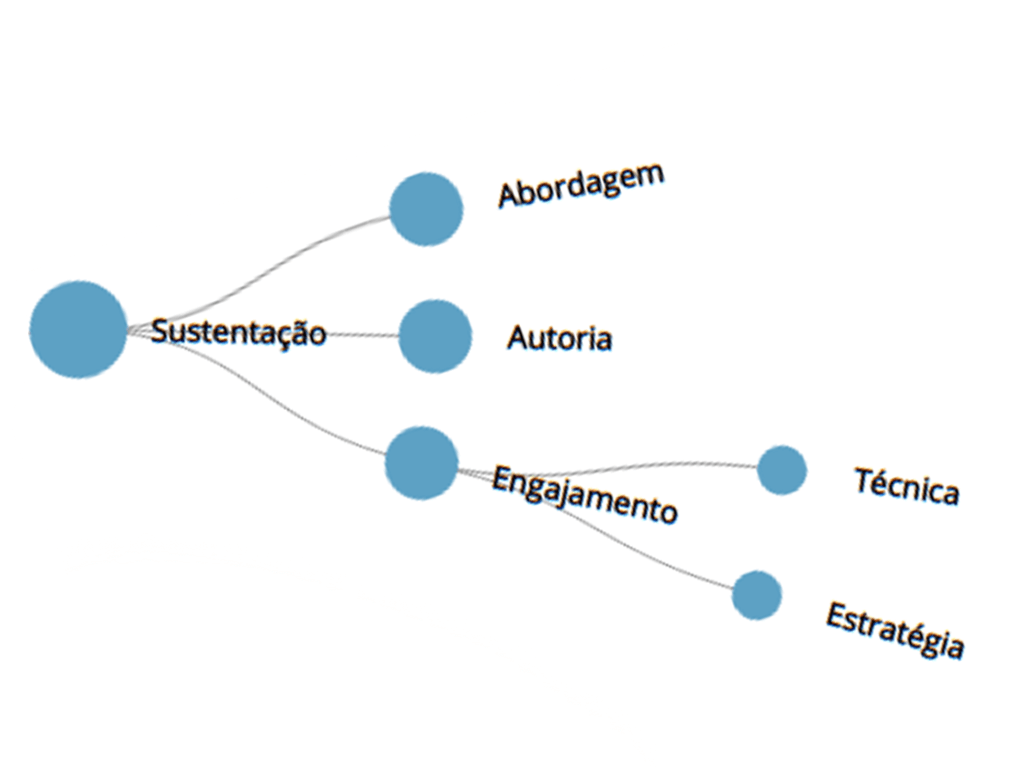
\includegraphics[scale=0.20]{./figuras/sustentacao.png}
    \caption{Hierarquia do grupo sustentação}
    \label{fig:grupo-sustentacao}
\end{figure}

\par
As definições das classe e subclasse desse grupo são representadas e descritas na Tabela \ref{tab:classesSustentacao}.

\begin{table}[!ht]
    \centering
    \caption{Classes e Subclasses do Grupo Sustentação}
    \label{tab:classesSustentacao}
    \begin{tabular}{l*{2}{>{\raggedright\arraybackslash}p{0.5\linewidth}}}
    \toprule
        Nome         & Descrição                       \\ 
    \midrule
        Abordagem    & Indica a origem da iniciativa.\\                         
        Autoria      & Informa quem é o responsável pelo desenvolvimento ou pela iniciativa da ferramenta.                \\
        Engajamento  & Indica se foi utilizada algum método específico na tentativa de aumentar o engajamento.         \\
        Técnica      & Refere-se à utilização de alguma técnica já estruturada para aumentar o engajamento dos usuários. \\
        Estratégia   & Diz respeito as ações realizadas na tentativa de aumentar o engajamento.\\
    \bottomrule
    \end{tabular}
\end{table}


%========================================================================================================================================================================================
\newpage
\subsubsection{Domínio}
\label{subsubsec:dominio}
O grupo domínio tem o objetivo de considerar características do ambiente em que a ferramenta está inserida. 
A figura \ref{fig:grupo-dominio} representa de forma visual as hierarquias definidas para o grupo.

\begin{figure}[!ht]
    \centering
    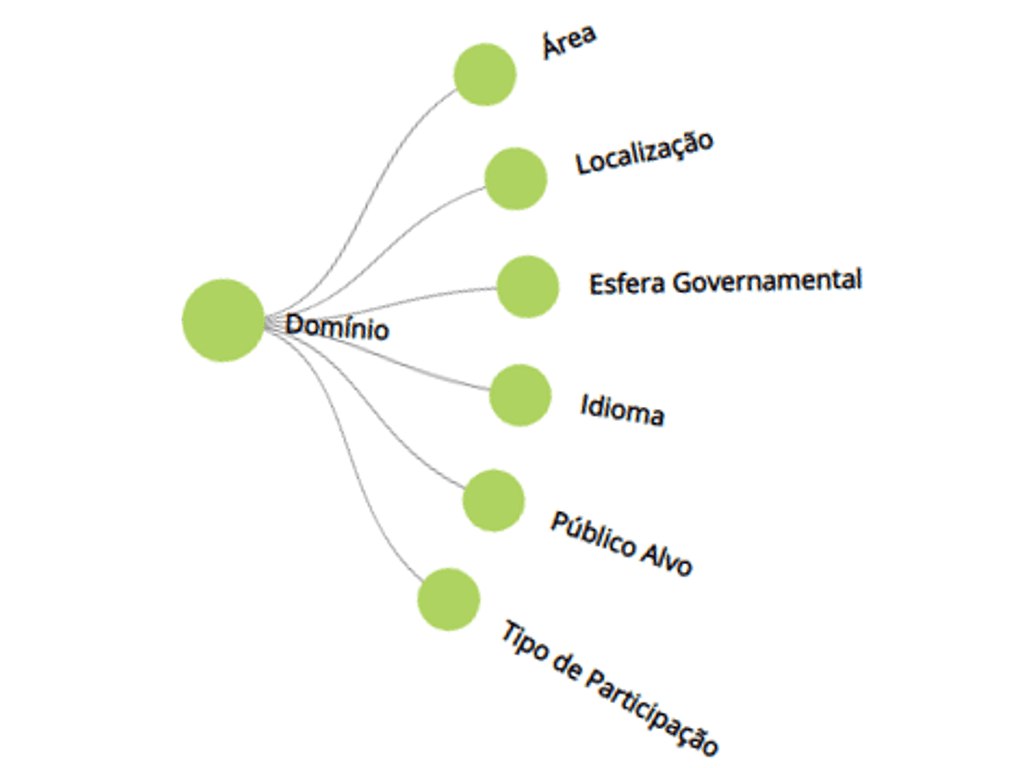
\includegraphics[scale=0.20]{./figuras/dominio.png}
    \caption{Hierarquia do grupo domínio}
    \label{fig:grupo-dominio}
\end{figure}

\par
As definições das classe e subclasse desse grupo são representadas e descritas na Tabela \ref{tab:classesDominio}.

\begin{table}[!ht]
    \centering
    \caption{Classes e Subclasses do Grupo Domínio}
    \label{tab:classesDominio}
    \begin{tabular}{l*{2}{>{\raggedright\arraybackslash}p{0.5\linewidth}}}
    \toprule
        Nome                  & Descrição \\ 
    \midrule
        Área                  & Indica se a ferramenta está inserida em alguma área específica da participação.\\                         
        Localização           & Informa se a ferramenta está inserida em um local geográfico específico e identifica qual o local.                \\
        Esfera governamental  & Identifica em qual nível da esfera governamental a ferramenta está inserida.       \\
        Idioma                & Informa em quais idiomas a ferramenta é disponibilizada.\\
        Público alvo          & Caracteriza qual público alvo que a ferramenta busca atingir e engajar.\\
        Tipo de participação  & Define se a participação é voluntária ou involuntária \\
    \bottomrule
    \end{tabular}
\end{table}

%========================================================================================================================================================================================
\newpage
\subsubsection{Tecnologias}
\label{subsubsec:tecnologias}
O grupo tecnologia contempla a análise sobre os aspectos técnicos utilizados nas ferramentas.
A figura \ref{fig:grupo-tecnologias} representa de forma visual as hierarquias definidas para o grupo.

\begin{figure}[!ht]
    \centering
    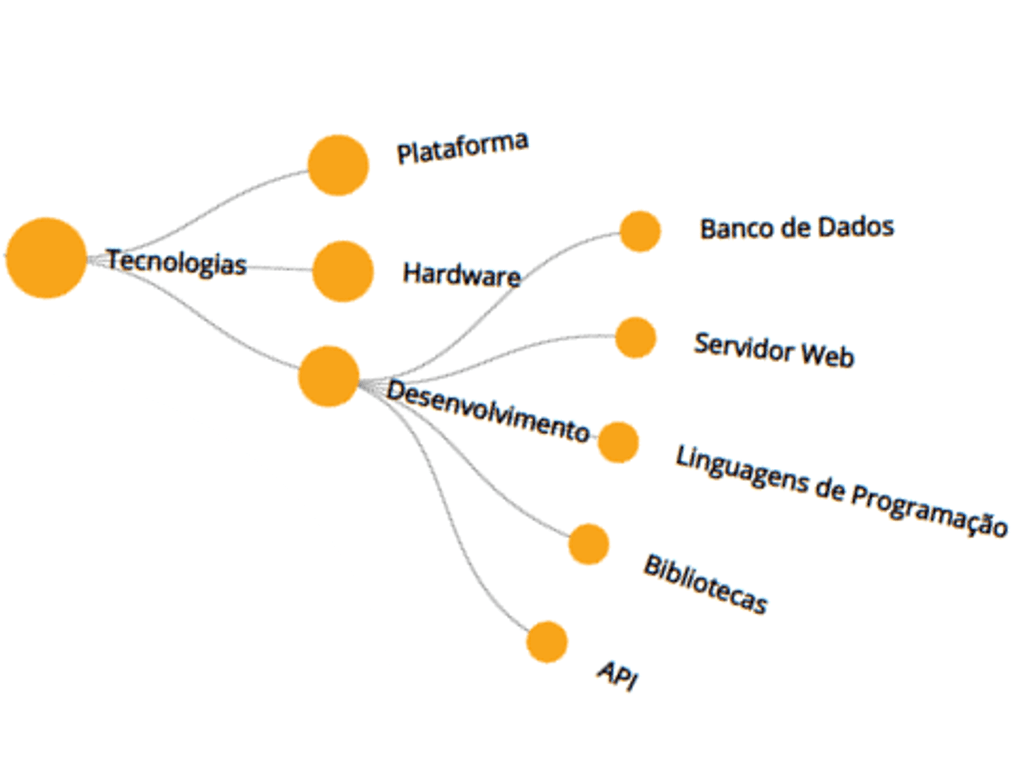
\includegraphics[scale=0.20]{./figuras/tecnologias.png}
    \caption{Hierarquia do grupo tecnologias}
    \label{fig:grupo-tecnologias}
\end{figure}

\par
As definições das classe e subclasse desse grupo são representadas e descritas na Tabela \ref{tab:classesTecnologias}.

\begin{table}[!ht]
    \centering
    \caption{Classes e Subclasses do Grupo Tecnologias}
    \label{tab:classesTecnologias}
    \begin{tabular}{l*{2}{>{\raggedright\arraybackslash}p{0.5\linewidth}}}
    \toprule
        Nome                      & Descrição \\ 
    \midrule
        Plataforma                & Indica em qual plataforma a ferramenta é disponibilizada.\\
        Hardware                  & Informa se a ferramenta utiliza algum hardware em sua implementação e qual hardware é esse.\\
        Desenvolvimento           & Descreve os itens associados aos recursos utilizados para o desenvolvimento da ferramenta. \\
        Banco de dados            & Refere-se ao uso de algum sistema de armazenamento de dados.\\
        Servidor web              & Indica se a ferramenta utiliza servidores e qual o tipo de servidor utilizado.\\
        Linguagens de Programação & Identifica quais linguagens foram utilizadas no desenvolvimento da ferramenta. \\
        Bibliotecas               & Indica se a ferramenta faz uso de alguma biblioteca de código.\\
        API                       & Informa se a ferramenta faz integração com alguma API. \\
    \bottomrule
    \end{tabular}
\end{table}

%========================================================================================================================================================================================
\newpage
\subsubsection{Funcionalidades}
\label{subsubsec:funcionalidades}
O grupo funcionalidades aborda as principais características de utilização disponibilizadas para interação com o usuário.
A hierarquia proposta para o grupo Tecnologias está representada na figura \ref{fig:grupo-funcionalidades}.

\begin{figure}[!ht]
    \centering
    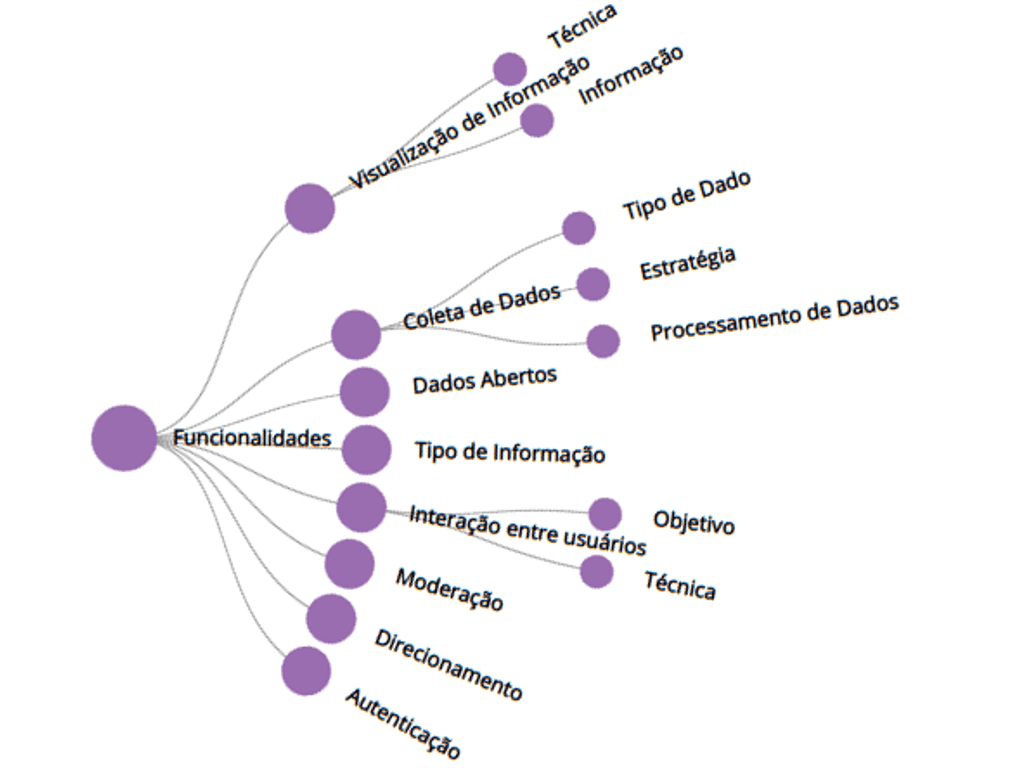
\includegraphics[scale=0.30]{./figuras/funcionalidades.png}
    \caption{Hierarquia do grupo funcionalidades}
    \label{fig:grupo-funcionalidades}
\end{figure}

\par
As definições das classe e subclasse desse grupo são representadas e descritas na Tabela \ref{tab:classesFuncionalidades}.

\begin{table}[!ht]
    \centering
    \caption{Classes e Subclasses do Grupo Funcionalidades}
    \label{tab:classesFuncionalidades}
    \begin{tabular}{l*{2}{>{\raggedright\arraybackslash}p{0.5\linewidth}}}
    \toprule
        Nome                       & Descrição \\ 
    \midrule
        Visualização de Informação & Indica se é utilizada alguma técnica de visualização para a apresentação das informações e quais informações são apresentadas pela ferramenta.\\
        Técnica                    & Refere-se à qual técnica de visualização é utilizada para representações gráficas.\\
        Informação                 & Diz respeito das informações que são disponibilizadas pelas visualizações.\\
        Coleta de Dados            & Define informações sobre os dados coletados e como são utilizados.\\
        Tipo de Dado               & Define os tipos de dados que são coletados.\\
        Estratégia                 & Relaciona-se a forma como os dados são coletados.\\
        Processamento de Dados     & Identifica se existe alguma forma de processamento sobre os dados.\\
        Dados abertos              & Indica se há a utilização de dados abertos, duas possibilidades podem ocorrer, os dados gerados pela ferramenta são disponibilizados em formato aberto, ou então, esses dados são utilizados para complementar alguma informação gerada pela ferramenta.\\
        Tipo de Informação         & Determina a respeito de que as informações na ferramenta tratam-se.\\
        Interação entre usuários   & Demonstra, para as aplicações que tem interação entre os usuários, qual o objetivo desta interação e qual a técnica utilizada.\\
        Objetivo                   & Refere-se ao objetivo da interação entre os usuários na aplicação.\\
        Técnica	                   & Define a forma como se dá a interação entre os usuários.\\
        Moderação                  & Apresenta quem é responsável por moderar as informações na ferramenta.\\
        Direcionamento             & Identifica quais ferramentas realizam encaminhamento de informações ao poder público.\\
        Autenticação               & Informa se existe a exigência de autenticação do usuário para utilizar a ferramenta.\\
    \bottomrule
    \end{tabular}
\end{table}
